\documentclass[1p]{elsarticle_modified}
%\bibliographystyle{elsarticle-num}

%\usepackage[colorlinks]{hyperref}
%\usepackage{abbrmath_seonhwa} %\Abb, \Ascr, \Acal ,\Abf, \Afrak
\usepackage{amsfonts}
\usepackage{amssymb}
\usepackage{amsmath}
\usepackage{amsthm}
\usepackage{scalefnt}
\usepackage{amsbsy}
\usepackage{kotex}
\usepackage{caption}
\usepackage{subfig}
\usepackage{color}
\usepackage{graphicx}
\usepackage{xcolor} %% white, black, red, green, blue, cyan, magenta, yellow
\usepackage{float}
\usepackage{setspace}
\usepackage{hyperref}

\usepackage{tikz}
\usetikzlibrary{arrows}

\usepackage{multirow}
\usepackage{array} % fixed length table
\usepackage{hhline}

%%%%%%%%%%%%%%%%%%%%%
\makeatletter
\renewcommand*\env@matrix[1][\arraystretch]{%
	\edef\arraystretch{#1}%
	\hskip -\arraycolsep
	\let\@ifnextchar\new@ifnextchar
	\array{*\c@MaxMatrixCols c}}
\makeatother %https://tex.stackexchange.com/questions/14071/how-can-i-increase-the-line-spacing-in-a-matrix
%%%%%%%%%%%%%%%

\usepackage[normalem]{ulem}

\newcommand{\msout}[1]{\ifmmode\text{\sout{\ensuremath{#1}}}\else\sout{#1}\fi}
%SOURCE: \msout is \stkout macro in https://tex.stackexchange.com/questions/20609/strikeout-in-math-mode

\newcommand{\cancel}[1]{
	\ifmmode
	{\color{red}\msout{#1}}
	\else
	{\color{red}\sout{#1}}
	\fi
}

\newcommand{\add}[1]{
	{\color{blue}\uwave{#1}}
}

\newcommand{\replace}[2]{
	\ifmmode
	{\color{red}\msout{#1}}{\color{blue}\uwave{#2}}
	\else
	{\color{red}\sout{#1}}{\color{blue}\uwave{#2}}
	\fi
}

\newcommand{\Sol}{\mathcal{S}} %segment
\newcommand{\D}{D} %diagram
\newcommand{\A}{\mathcal{A}} %arc


%%%%%%%%%%%%%%%%%%%%%%%%%%%%%5 test

\def\sl{\operatorname{\textup{SL}}(2,\Cbb)}
\def\psl{\operatorname{\textup{PSL}}(2,\Cbb)}
\def\quan{\mkern 1mu \triangleright \mkern 1mu}

\theoremstyle{definition}
\newtheorem{thm}{Theorem}[section]
\newtheorem{prop}[thm]{Proposition}
\newtheorem{lem}[thm]{Lemma}
\newtheorem{ques}[thm]{Question}
\newtheorem{cor}[thm]{Corollary}
\newtheorem{defn}[thm]{Definition}
\newtheorem{exam}[thm]{Example}
\newtheorem{rmk}[thm]{Remark}
\newtheorem{alg}[thm]{Algorithm}

\newcommand{\I}{\sqrt{-1}}
\begin{document}

%\begin{frontmatter}
%
%\title{Boundary parabolic representations of knots up to 8 crossings}
%
%%% Group authors per affiliation:
%\author{Yunhi Cho} 
%\address{Department of Mathematics, University of Seoul, Seoul, Korea}
%\ead{yhcho@uos.ac.kr}
%
%
%\author{Seonhwa Kim} %\fnref{s_kim}}
%\address{Center for Geometry and Physics, Institute for Basic Science, Pohang, 37673, Korea}
%\ead{ryeona17@ibs.re.kr}
%
%\author{Hyuk Kim}
%\address{Department of Mathematical Sciences, Seoul National University, Seoul 08826, Korea}
%\ead{hyukkim@snu.ac.kr}
%
%\author{Seokbeom Yoon}
%\address{Department of Mathematical Sciences, Seoul National University, Seoul, 08826,  Korea}
%\ead{sbyoon15@snu.ac.kr}
%
%\begin{abstract}
%We find all boundary parabolic representation of knots up to 8 crossings.
%
%\end{abstract}
%\begin{keyword}
%    \MSC[2010] 57M25 
%\end{keyword}
%
%\end{frontmatter}

%\linenumbers
%\tableofcontents
%
\newcommand\colored[1]{\textcolor{white}{\rule[-0.35ex]{0.8em}{1.4ex}}\kern-0.8em\color{red} #1}%
%\newcommand\colored[1]{\textcolor{white}{ #1}\kern-2.17ex	\textcolor{white}{ #1}\kern-1.81ex	\textcolor{white}{ #1}\kern-2.15ex\color{red}#1	}

{\Large $\underline{11a_{6}~(K11a_{6})}$}

\setlength{\tabcolsep}{10pt}
\renewcommand{\arraystretch}{1.6}
\vspace{1cm}\begin{tabular}{m{100pt}>{\centering\arraybackslash}m{274pt}}
\multirow{5}{120pt}{
	\centering
	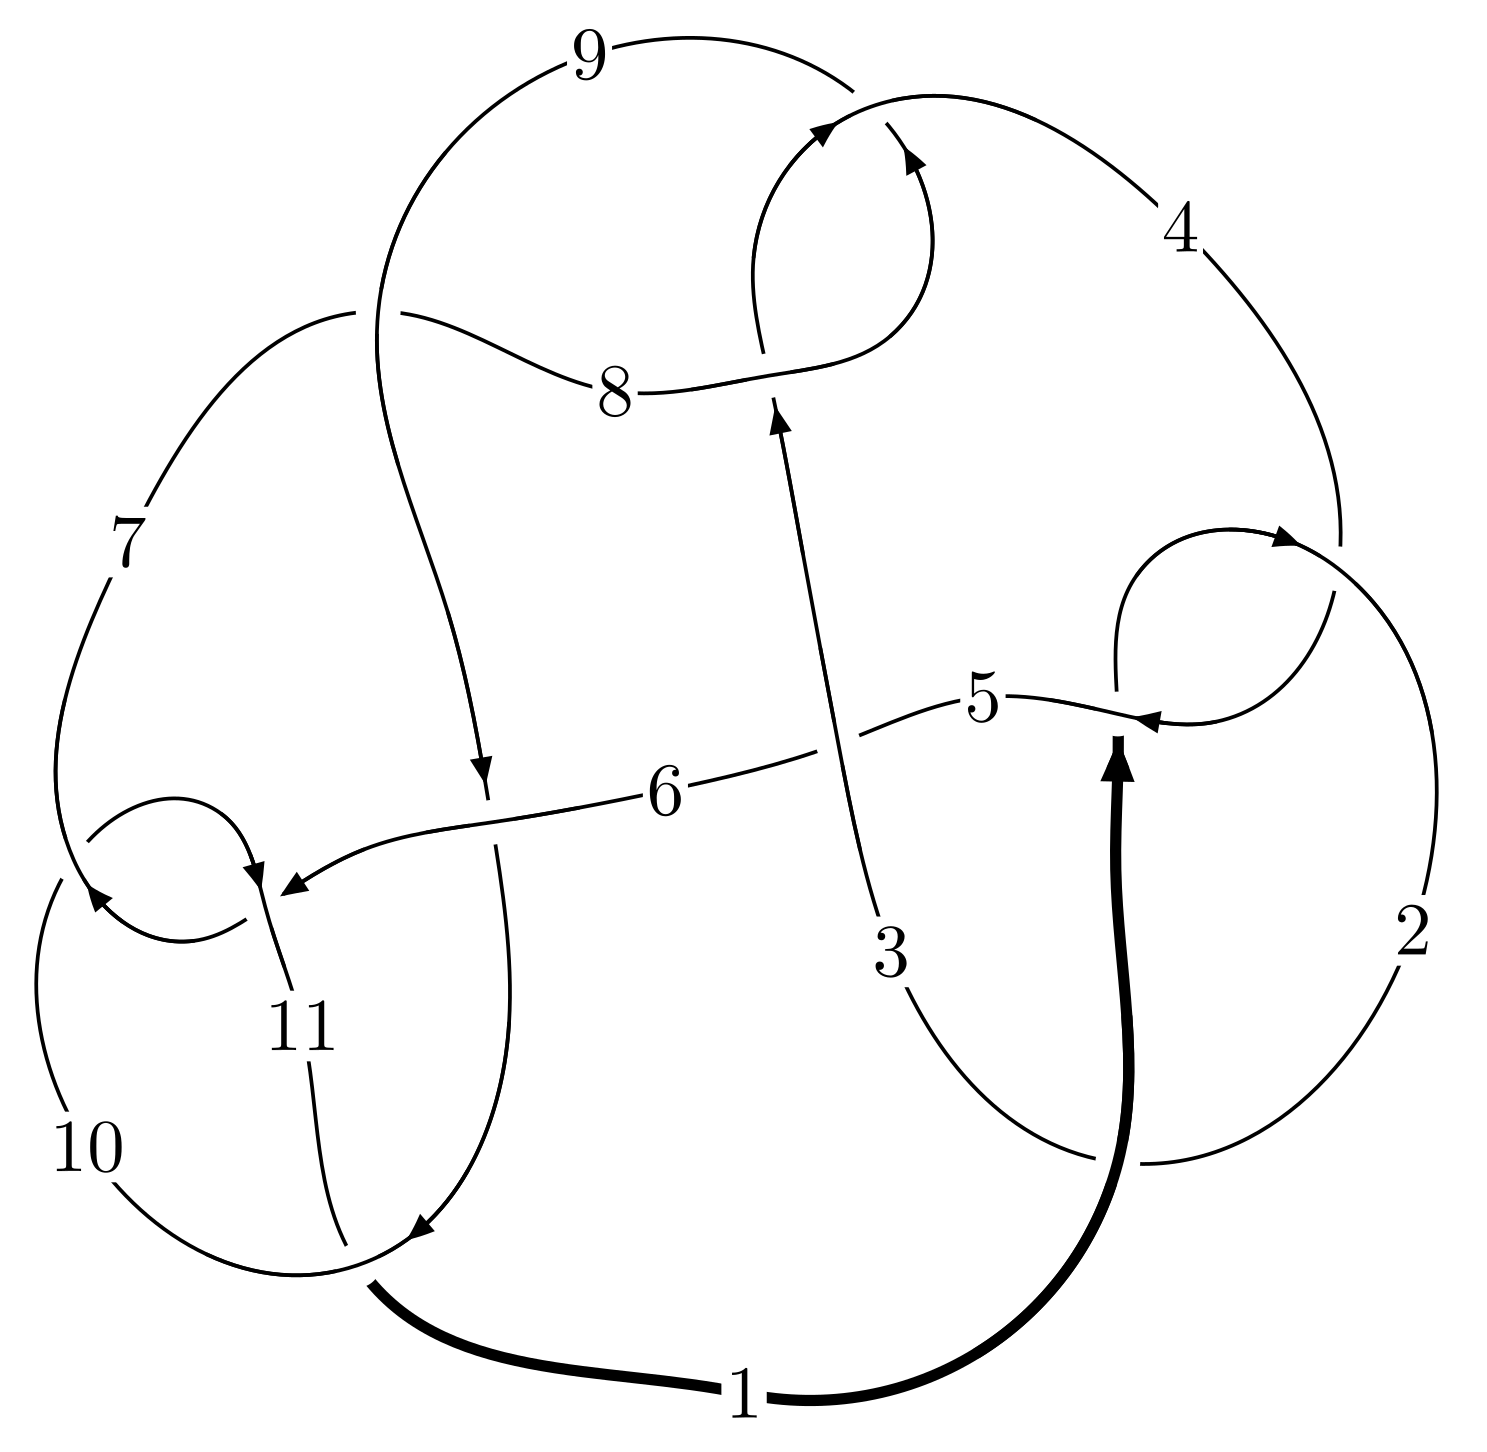
\includegraphics[width=112pt]{../../../GIT/diagram.site/Diagrams/png/255_11a_6.png}\\
\ \ \ A knot diagram\footnotemark}&
\allowdisplaybreaks
\textbf{Linearized knot diagam} \\
\cline{2-2}
 &
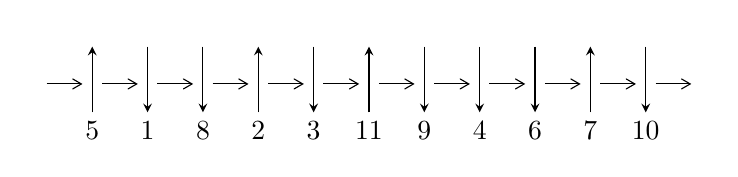
\begin{tikzpicture}[x=20pt, y=17pt]
	% nodes
	\node (C0) at (0, 0) {};
	\node (C1) at (1, 0) {};
	\node (C1U) at (1, +1) {};
	\node (C1D) at (1, -1) {5};

	\node (C2) at (2, 0) {};
	\node (C2U) at (2, +1) {};
	\node (C2D) at (2, -1) {1};

	\node (C3) at (3, 0) {};
	\node (C3U) at (3, +1) {};
	\node (C3D) at (3, -1) {8};

	\node (C4) at (4, 0) {};
	\node (C4U) at (4, +1) {};
	\node (C4D) at (4, -1) {2};

	\node (C5) at (5, 0) {};
	\node (C5U) at (5, +1) {};
	\node (C5D) at (5, -1) {3};

	\node (C6) at (6, 0) {};
	\node (C6U) at (6, +1) {};
	\node (C6D) at (6, -1) {11};

	\node (C7) at (7, 0) {};
	\node (C7U) at (7, +1) {};
	\node (C7D) at (7, -1) {9};

	\node (C8) at (8, 0) {};
	\node (C8U) at (8, +1) {};
	\node (C8D) at (8, -1) {4};

	\node (C9) at (9, 0) {};
	\node (C9U) at (9, +1) {};
	\node (C9D) at (9, -1) {6};

	\node (C10) at (10, 0) {};
	\node (C10U) at (10, +1) {};
	\node (C10D) at (10, -1) {7};

	\node (C11) at (11, 0) {};
	\node (C11U) at (11, +1) {};
	\node (C11D) at (11, -1) {10};
	\node (C12) at (12, 0) {};

	% arrows
	\draw[->,>={angle 60}]
	(C0) edge (C1) (C1) edge (C2) (C2) edge (C3) (C3) edge (C4) (C4) edge (C5) (C5) edge (C6) (C6) edge (C7) (C7) edge (C8) (C8) edge (C9) (C9) edge (C10) (C10) edge (C11) (C11) edge (C12) ;	\draw[->,>=stealth]
	(C1D) edge (C1U) (C2U) edge (C2D) (C3U) edge (C3D) (C4D) edge (C4U) (C5U) edge (C5D) (C6D) edge (C6U) (C7U) edge (C7D) (C8U) edge (C8D) (C9U) edge (C9D) (C10D) edge (C10U) (C11U) edge (C11D) ;
	\end{tikzpicture} \\
\hhline{~~} \\& 
\textbf{Solving Sequence} \\ \cline{2-2} 
 &
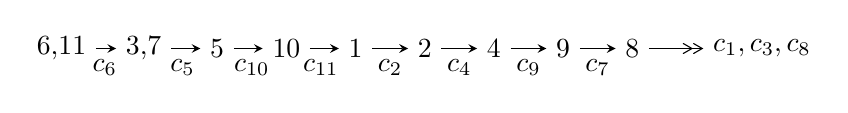
\begin{tikzpicture}[x=25pt, y=7pt]
	% node
	\node (A0) at (-1/8, 0) {6,11};
	\node (A1) at (17/16, 0) {3,7};
	\node (A2) at (17/8, 0) {5};
	\node (A3) at (25/8, 0) {10};
	\node (A4) at (33/8, 0) {1};
	\node (A5) at (41/8, 0) {2};
	\node (A6) at (49/8, 0) {4};
	\node (A7) at (57/8, 0) {9};
	\node (A8) at (65/8, 0) {8};
	\node (C1) at (1/2, -1) {$c_{6}$};
	\node (C2) at (13/8, -1) {$c_{5}$};
	\node (C3) at (21/8, -1) {$c_{10}$};
	\node (C4) at (29/8, -1) {$c_{11}$};
	\node (C5) at (37/8, -1) {$c_{2}$};
	\node (C6) at (45/8, -1) {$c_{4}$};
	\node (C7) at (53/8, -1) {$c_{9}$};
	\node (C8) at (61/8, -1) {$c_{7}$};
	\node (A9) at (10, 0) {$c_{1},c_{3},c_{8}$};

	% edge
	\draw[->,>=stealth]	
	(A0) edge (A1) (A1) edge (A2) (A2) edge (A3) (A3) edge (A4) (A4) edge (A5) (A5) edge (A6) (A6) edge (A7) (A7) edge (A8) ;
	\draw[->>,>={angle 60}]	
	(A8) edge (A9);
\end{tikzpicture} \\ 

\end{tabular} \\

\footnotetext{
The image of knot diagram is generated by the software ``\textbf{Draw programme}" developed by Andrew Bartholomew(\url{http://www.layer8.co.uk/maths/draw/index.htm\#Running-draw}), where we modified some parts for our purpose(\url{https://github.com/CATsTAILs/LinksPainter}).
}\phantom \\ \newline 
\centering \textbf{Ideals for irreducible components\footnotemark of $X_{\text{par}}$} 
 
\begin{align*}
I^u_{1}&=\langle 
- u^3+b- u,\;- u^{13}- u^{12}-4 u^{11}-3 u^{10}-7 u^9-5 u^8-6 u^7-4 u^6-2 u^5-2 u^4-2 u^3- u^2+a-2 u-1,\\
\phantom{I^u_{1}}&\phantom{= \langle  }u^{17}+u^{16}+\cdots+u+1\rangle \\
I^u_{2}&=\langle 
- u^{53}-2 u^{52}+\cdots+b-1,\;- u^{52}-2 u^{51}+\cdots+a-3,\;u^{54}+2 u^{53}+\cdots+u+1\rangle \\
I^u_{3}&=\langle 
b+u+1,\;a+1,\;u^2+u+1\rangle \\
I^u_{4}&=\langle 
b- u,\;a- u-1,\;u^2+u+1\rangle \\
\\
\end{align*}
\raggedright * 4 irreducible components of $\dim_{\mathbb{C}}=0$, with total 75 representations.\\
\footnotetext{All coefficients of polynomials are rational numbers. But the coefficients are sometimes approximated in decimal forms when there is not enough margin.}
\newpage
\renewcommand{\arraystretch}{1}
\centering \section*{I. $I^u_{1}= \langle - u^3+b- u,\;- u^{13}- u^{12}+\cdots+a-1,\;u^{17}+u^{16}+\cdots+u+1 \rangle$}
\flushleft \textbf{(i) Arc colorings}\\
\begin{tabular}{m{7pt} m{180pt} m{7pt} m{180pt} }
\flushright $a_{6}=$&$\begin{pmatrix}1\\0\end{pmatrix}$ \\
\flushright $a_{11}=$&$\begin{pmatrix}0\\u\end{pmatrix}$ \\
\flushright $a_{3}=$&$\begin{pmatrix}u^{13}+u^{12}+\cdots+2 u+1\\u^3+u\end{pmatrix}$ \\
\flushright $a_{7}=$&$\begin{pmatrix}1\\- u^2\end{pmatrix}$ \\
\flushright $a_{5}=$&$\begin{pmatrix}- u^{16}- u^{15}+\cdots- u+1\\- u^6-2 u^4- u^2\end{pmatrix}$ \\
\flushright $a_{10}=$&$\begin{pmatrix}- u\\u^3+u\end{pmatrix}$ \\
\flushright $a_{1}=$&$\begin{pmatrix}- u^3\\u^5+u^3+u\end{pmatrix}$ \\
\flushright $a_{2}=$&$\begin{pmatrix}u^{13}+u^{12}+\cdots+2 u+1\\- u^7- u^5+u\end{pmatrix}$ \\
\flushright $a_{4}=$&$\begin{pmatrix}- u^{16}- u^{15}+\cdots- u^3+1\\- u^8-2 u^6-2 u^4\end{pmatrix}$ \\
\flushright $a_{9}=$&$\begin{pmatrix}u^3\\u^3+u\end{pmatrix}$ \\
\flushright $a_{8}=$&$\begin{pmatrix}u^8+u^6+u^4+1\\u^8+2 u^6+2 u^4\end{pmatrix}$\\ \flushright $a_{8}=$&$\begin{pmatrix}u^8+u^6+u^4+1\\u^8+2 u^6+2 u^4\end{pmatrix}$\\&\end{tabular}
\flushleft \textbf{(ii) Obstruction class $= -1$}\\~\\
\flushleft \textbf{(iii) Cusp Shapes $= -4 u^{16}-6 u^{15}-18 u^{14}-22 u^{13}-40 u^{12}-46 u^{11}-56 u^{10}-54 u^9-54 u^8-44 u^7-44 u^6-28 u^5-26 u^4-22 u^3-12 u^2-10 u-8$}\\~\\
\newpage\renewcommand{\arraystretch}{1}
\flushleft \textbf{(iv) u-Polynomials at the component}\newline \\
\begin{tabular}{m{50pt}|m{274pt}}
Crossings & \hspace{64pt}u-Polynomials at each crossing \\
\hline $$\begin{aligned}c_{1},c_{4},c_{6}\\c_{10}\end{aligned}$$&$\begin{aligned}
&u^{17}+u^{16}+\cdots+u+1
\end{aligned}$\\
\hline $$\begin{aligned}c_{2},c_{11}\end{aligned}$$&$\begin{aligned}
&u^{17}+9 u^{16}+\cdots-3 u-1
\end{aligned}$\\
\hline $$\begin{aligned}c_{3},c_{8}\end{aligned}$$&$\begin{aligned}
&u^{17}-5 u^{16}+\cdots-8 u+4
\end{aligned}$\\
\hline $$\begin{aligned}c_{5},c_{9}\end{aligned}$$&$\begin{aligned}
&u^{17}- u^{16}+\cdots- u+2
\end{aligned}$\\
\hline $$\begin{aligned}c_{7}\end{aligned}$$&$\begin{aligned}
&u^{17}+5 u^{16}+\cdots+56 u^2+16
\end{aligned}$\\
\hline
\end{tabular}\\~\\
\newpage\renewcommand{\arraystretch}{1}
\flushleft \textbf{(v) Riley Polynomials at the component}\newline \\
\begin{tabular}{m{50pt}|m{274pt}}
Crossings & \hspace{64pt}Riley Polynomials at each crossing \\
\hline $$\begin{aligned}c_{1},c_{4},c_{6}\\c_{10}\end{aligned}$$&$\begin{aligned}
&y^{17}+9 y^{16}+\cdots-3 y-1
\end{aligned}$\\
\hline $$\begin{aligned}c_{2},c_{11}\end{aligned}$$&$\begin{aligned}
&y^{17}+y^{16}+\cdots+5 y-1
\end{aligned}$\\
\hline $$\begin{aligned}c_{3},c_{8}\end{aligned}$$&$\begin{aligned}
&y^{17}-5 y^{16}+\cdots-56 y^2-16
\end{aligned}$\\
\hline $$\begin{aligned}c_{5},c_{9}\end{aligned}$$&$\begin{aligned}
&y^{17}-7 y^{16}+\cdots+y-4
\end{aligned}$\\
\hline $$\begin{aligned}c_{7}\end{aligned}$$&$\begin{aligned}
&y^{17}+7 y^{16}+\cdots-1792 y-256
\end{aligned}$\\
\hline
\end{tabular}\\~\\
\newpage\flushleft \textbf{(vi) Complex Volumes and Cusp Shapes}
$$\begin{array}{c|c|c}  
\text{Solutions to }I^u_{1}& \I (\text{vol} + \sqrt{-1}CS) & \text{Cusp shape}\\
 \hline 
\begin{aligned}
u &= \phantom{-}0.364031 + 1.042940 I \\
a &= -2.23442 + 1.04009 I \\
b &= -0.775626 + 0.323135 I\end{aligned}
 & -3.22508 + 4.12748 I & -8.88917 - 5.53460 I \\ \hline\begin{aligned}
u &= \phantom{-}0.364031 - 1.042940 I \\
a &= -2.23442 - 1.04009 I \\
b &= -0.775626 - 0.323135 I\end{aligned}
 & -3.22508 - 4.12748 I & -8.88917 + 5.53460 I \\ \hline\begin{aligned}
u &= -0.783861 + 0.397949 I \\
a &= -0.183240 - 0.678603 I \\
b &= -0.893091 + 1.068470 I\end{aligned}
 & \phantom{-}2.83523 + 5.37992 I & \phantom{-}0.58832 - 3.10862 I \\ \hline\begin{aligned}
u &= -0.783861 - 0.397949 I \\
a &= -0.183240 + 0.678603 I \\
b &= -0.893091 - 1.068470 I\end{aligned}
 & \phantom{-}2.83523 - 5.37992 I & \phantom{-}0.58832 + 3.10862 I \\ \hline\begin{aligned}
u &= -0.228107 + 1.129710 I \\
a &= \phantom{-}1.006760 + 0.533745 I \\
b &= \phantom{-}0.633379 - 0.135717 I\end{aligned}
 & -6.66052 + 0.33441 I & -12.27972 + 0.14725 I \\ \hline\begin{aligned}
u &= -0.228107 - 1.129710 I \\
a &= \phantom{-}1.006760 - 0.533745 I \\
b &= \phantom{-}0.633379 + 0.135717 I\end{aligned}
 & -6.66052 - 0.33441 I & -12.27972 - 0.14725 I \\ \hline\begin{aligned}
u &= \phantom{-}0.701375 + 0.463501 I \\
a &= \phantom{-}0.486517 - 0.757070 I \\
b &= \phantom{-}0.594363 + 1.047950 I\end{aligned}
 & \phantom{-}3.82884 + 0.36538 I & \phantom{-}2.43059 - 2.03934 I \\ \hline\begin{aligned}
u &= \phantom{-}0.701375 - 0.463501 I \\
a &= \phantom{-}0.486517 + 0.757070 I \\
b &= \phantom{-}0.594363 - 1.047950 I\end{aligned}
 & \phantom{-}3.82884 - 0.36538 I & \phantom{-}2.43059 + 2.03934 I \\ \hline\begin{aligned}
u &= \phantom{-}0.572214 + 1.088100 I \\
a &= -2.74846 - 1.45002 I \\
b &= -1.27288 + 0.86865 I\end{aligned}
 & \phantom{-}0.06925 + 9.48553 I & -4.16847 - 7.65622 I \\ \hline\begin{aligned}
u &= \phantom{-}0.572214 - 1.088100 I \\
a &= -2.74846 + 1.45002 I \\
b &= -1.27288 - 0.86865 I\end{aligned}
 & \phantom{-}0.06925 - 9.48553 I & -4.16847 + 7.65622 I\\
 \hline 
 \end{array}$$\newpage$$\begin{array}{c|c|c}  
\text{Solutions to }I^u_{1}& \I (\text{vol} + \sqrt{-1}CS) & \text{Cusp shape}\\
 \hline 
\begin{aligned}
u &= -0.451021 + 1.148490 I \\
a &= \phantom{-}2.21759 - 0.36414 I \\
b &= \phantom{-}1.241950 + 0.334481 I\end{aligned}
 & -8.03366 - 8.05681 I & -11.19202 + 7.52466 I \\ \hline\begin{aligned}
u &= -0.451021 - 1.148490 I \\
a &= \phantom{-}2.21759 + 0.36414 I \\
b &= \phantom{-}1.241950 - 0.334481 I\end{aligned}
 & -8.03366 + 8.05681 I & -11.19202 - 7.52466 I \\ \hline\begin{aligned}
u &= -0.601205 + 1.123530 I \\
a &= \phantom{-}2.35978 - 1.49796 I \\
b &= \phantom{-}1.45822 + 0.92357 I\end{aligned}
 & -1.4738 - 15.8440 I & -5.36436 + 10.86165 I \\ \hline\begin{aligned}
u &= -0.601205 - 1.123530 I \\
a &= \phantom{-}2.35978 + 1.49796 I \\
b &= \phantom{-}1.45822 - 0.92357 I\end{aligned}
 & -1.4738 + 15.8440 I & -5.36436 - 10.86165 I \\ \hline\begin{aligned}
u &= \phantom{-}0.237306 + 0.655876 I \\
a &= \phantom{-}0.689506 + 1.196060 I \\
b &= -0.055578 + 0.484541 I\end{aligned}
 & -0.38141 + 1.45461 I & -4.03529 - 4.09951 I \\ \hline\begin{aligned}
u &= \phantom{-}0.237306 - 0.655876 I \\
a &= \phantom{-}0.689506 - 1.196060 I \\
b &= -0.055578 - 0.484541 I\end{aligned}
 & -0.38141 - 1.45461 I & -4.03529 + 4.09951 I \\ \hline\begin{aligned}
u &= -0.621462\phantom{ +0.000000I} \\
a &= -0.188062\phantom{ +0.000000I} \\
b &= -0.861480\phantom{ +0.000000I}\end{aligned}
 & -1.88169\phantom{ +0.000000I} & -4.17970\phantom{ +0.000000I}\\
 \hline 
 \end{array}$$\newpage\newpage\renewcommand{\arraystretch}{1}
\centering \section*{II. $I^u_{2}= \langle - u^{53}-2 u^{52}+\cdots+b-1,\;- u^{52}-2 u^{51}+\cdots+a-3,\;u^{54}+2 u^{53}+\cdots+u+1 \rangle$}
\flushleft \textbf{(i) Arc colorings}\\
\begin{tabular}{m{7pt} m{180pt} m{7pt} m{180pt} }
\flushright $a_{6}=$&$\begin{pmatrix}1\\0\end{pmatrix}$ \\
\flushright $a_{11}=$&$\begin{pmatrix}0\\u\end{pmatrix}$ \\
\flushright $a_{3}=$&$\begin{pmatrix}u^{52}+2 u^{51}+\cdots+3 u+3\\u^{53}+2 u^{52}+\cdots+3 u+1\end{pmatrix}$ \\
\flushright $a_{7}=$&$\begin{pmatrix}1\\- u^2\end{pmatrix}$ \\
\flushright $a_{5}=$&$\begin{pmatrix}u^{52}+u^{51}+\cdots+u+3\\u^{53}+2 u^{52}+\cdots+2 u+1\end{pmatrix}$ \\
\flushright $a_{10}=$&$\begin{pmatrix}- u\\u^3+u\end{pmatrix}$ \\
\flushright $a_{1}=$&$\begin{pmatrix}- u^3\\u^5+u^3+u\end{pmatrix}$ \\
\flushright $a_{2}=$&$\begin{pmatrix}- u^{53}+u^{52}+\cdots+3 u+4\\u^{53}+4 u^{52}+\cdots+4 u+3\end{pmatrix}$ \\
\flushright $a_{4}=$&$\begin{pmatrix}-2 u^{53}- u^{52}+\cdots+u+3\\u^{53}+4 u^{52}+\cdots+3 u+3\end{pmatrix}$ \\
\flushright $a_{9}=$&$\begin{pmatrix}u^3\\u^3+u\end{pmatrix}$ \\
\flushright $a_{8}=$&$\begin{pmatrix}u^8+u^6+u^4+1\\u^8+2 u^6+2 u^4\end{pmatrix}$\\ \flushright $a_{8}=$&$\begin{pmatrix}u^8+u^6+u^4+1\\u^8+2 u^6+2 u^4\end{pmatrix}$\\&\end{tabular}
\flushleft \textbf{(ii) Obstruction class $= -1$}\\~\\
\flushleft \textbf{(iii) Cusp Shapes $= -5 u^{53}-8 u^{52}+\cdots-15 u-5$}\\~\\
\newpage\renewcommand{\arraystretch}{1}
\flushleft \textbf{(iv) u-Polynomials at the component}\newline \\
\begin{tabular}{m{50pt}|m{274pt}}
Crossings & \hspace{64pt}u-Polynomials at each crossing \\
\hline $$\begin{aligned}c_{1},c_{4},c_{6}\\c_{10}\end{aligned}$$&$\begin{aligned}
&u^{54}+2 u^{53}+\cdots+u+1
\end{aligned}$\\
\hline $$\begin{aligned}c_{2},c_{11}\end{aligned}$$&$\begin{aligned}
&u^{54}+24 u^{53}+\cdots+5 u+1
\end{aligned}$\\
\hline $$\begin{aligned}c_{3},c_{8}\end{aligned}$$&$\begin{aligned}
&(u^{27}+2 u^{26}+\cdots+3 u+2)^{2}
\end{aligned}$\\
\hline $$\begin{aligned}c_{5},c_{9}\end{aligned}$$&$\begin{aligned}
&u^{54}-2 u^{53}+\cdots-145 u+17
\end{aligned}$\\
\hline $$\begin{aligned}c_{7}\end{aligned}$$&$\begin{aligned}
&(u^{27}+10 u^{26}+\cdots+25 u+4)^{2}
\end{aligned}$\\
\hline
\end{tabular}\\~\\
\newpage\renewcommand{\arraystretch}{1}
\flushleft \textbf{(v) Riley Polynomials at the component}\newline \\
\begin{tabular}{m{50pt}|m{274pt}}
Crossings & \hspace{64pt}Riley Polynomials at each crossing \\
\hline $$\begin{aligned}c_{1},c_{4},c_{6}\\c_{10}\end{aligned}$$&$\begin{aligned}
&y^{54}+24 y^{53}+\cdots+5 y+1
\end{aligned}$\\
\hline $$\begin{aligned}c_{2},c_{11}\end{aligned}$$&$\begin{aligned}
&y^{54}+12 y^{53}+\cdots+53 y+1
\end{aligned}$\\
\hline $$\begin{aligned}c_{3},c_{8}\end{aligned}$$&$\begin{aligned}
&(y^{27}-10 y^{26}+\cdots+25 y-4)^{2}
\end{aligned}$\\
\hline $$\begin{aligned}c_{5},c_{9}\end{aligned}$$&$\begin{aligned}
&y^{54}+38 y^{52}+\cdots-4637 y+289
\end{aligned}$\\
\hline $$\begin{aligned}c_{7}\end{aligned}$$&$\begin{aligned}
&(y^{27}+14 y^{26}+\cdots-95 y-16)^{2}
\end{aligned}$\\
\hline
\end{tabular}\\~\\
\newpage\flushleft \textbf{(vi) Complex Volumes and Cusp Shapes}
$$\begin{array}{c|c|c}  
\text{Solutions to }I^u_{2}& \I (\text{vol} + \sqrt{-1}CS) & \text{Cusp shape}\\
 \hline 
\begin{aligned}
u &= -0.349223 + 0.956682 I \\
a &= -1.49999 - 0.14653 I \\
b &= -0.583952 - 1.234060 I\end{aligned}
 & -1.01872 - 3.73043 I & -9.17515 + 3.57270 I \\ \hline\begin{aligned}
u &= -0.349223 - 0.956682 I \\
a &= -1.49999 + 0.14653 I \\
b &= -0.583952 + 1.234060 I\end{aligned}
 & -1.01872 + 3.73043 I & -9.17515 - 3.57270 I \\ \hline\begin{aligned}
u &= \phantom{-}0.748850 + 0.603065 I \\
a &= \phantom{-}0.217497 + 0.802869 I \\
b &= \phantom{-}1.22625 - 0.91458 I\end{aligned}
 & \phantom{-}1.90449 + 7.58447 I & -1.82775 - 8.11380 I \\ \hline\begin{aligned}
u &= \phantom{-}0.748850 - 0.603065 I \\
a &= \phantom{-}0.217497 - 0.802869 I \\
b &= \phantom{-}1.22625 + 0.91458 I\end{aligned}
 & \phantom{-}1.90449 - 7.58447 I & -1.82775 + 8.11380 I \\ \hline\begin{aligned}
u &= -0.239448 + 0.923216 I \\
a &= \phantom{-}0.896353 + 0.856395 I \\
b &= -0.055765 + 1.171120 I\end{aligned}
 & -0.538859 + 1.164110 I & -6.09920 - 3.89817 I \\ \hline\begin{aligned}
u &= -0.239448 - 0.923216 I \\
a &= \phantom{-}0.896353 - 0.856395 I \\
b &= -0.055765 - 1.171120 I\end{aligned}
 & -0.538859 - 1.164110 I & -6.09920 + 3.89817 I \\ \hline\begin{aligned}
u &= \phantom{-}0.227574 + 1.026590 I \\
a &= -2.62355 - 1.10867 I \\
b &= -1.066100 - 0.705684 I\end{aligned}
 & -2.23363 - 2.56106 I & -7.40701 + 2.25118 I \\ \hline\begin{aligned}
u &= \phantom{-}0.227574 - 1.026590 I \\
a &= -2.62355 + 1.10867 I \\
b &= -1.066100 + 0.705684 I\end{aligned}
 & -2.23363 + 2.56106 I & -7.40701 - 2.25118 I \\ \hline\begin{aligned}
u &= \phantom{-}0.622213 + 0.701611 I \\
a &= -0.125307 + 0.872732 I \\
b &= \phantom{-}0.359087 + 0.295131 I\end{aligned}
 & -0.538859 + 1.164110 I & -6.09920 - 3.89817 I \\ \hline\begin{aligned}
u &= \phantom{-}0.622213 - 0.701611 I \\
a &= -0.125307 - 0.872732 I \\
b &= \phantom{-}0.359087 - 0.295131 I\end{aligned}
 & -0.538859 - 1.164110 I & -6.09920 + 3.89817 I\\
 \hline 
 \end{array}$$\newpage$$\begin{array}{c|c|c}  
\text{Solutions to }I^u_{2}& \I (\text{vol} + \sqrt{-1}CS) & \text{Cusp shape}\\
 \hline 
\begin{aligned}
u &= \phantom{-}0.725685 + 0.567873 I \\
a &= -0.020644 - 0.712194 I \\
b &= -0.639257 + 1.031450 I\end{aligned}
 & \phantom{-}3.74831 + 2.63920 I & \phantom{-}1.74271 - 3.37289 I \\ \hline\begin{aligned}
u &= \phantom{-}0.725685 - 0.567873 I \\
a &= -0.020644 + 0.712194 I \\
b &= -0.639257 - 1.031450 I\end{aligned}
 & \phantom{-}3.74831 - 2.63920 I & \phantom{-}1.74271 + 3.37289 I \\ \hline\begin{aligned}
u &= \phantom{-}0.626309 + 0.880271 I \\
a &= \phantom{-}0.459060 - 0.105789 I \\
b &= \phantom{-}0.567055 - 0.431109 I\end{aligned}
 & -1.01872 + 3.73043 I & -9.17515 - 3.57270 I \\ \hline\begin{aligned}
u &= \phantom{-}0.626309 - 0.880271 I \\
a &= \phantom{-}0.459060 + 0.105789 I \\
b &= \phantom{-}0.567055 + 0.431109 I\end{aligned}
 & -1.01872 - 3.73043 I & -9.17515 + 3.57270 I \\ \hline\begin{aligned}
u &= \phantom{-}0.312561 + 0.860769 I \\
a &= \phantom{-}1.090150 + 0.590870 I \\
b &= \phantom{-}0.301084 + 0.372364 I\end{aligned}
 & -0.36265 + 1.51655 I & -2.55288 - 3.58996 I \\ \hline\begin{aligned}
u &= \phantom{-}0.312561 - 0.860769 I \\
a &= \phantom{-}1.090150 - 0.590870 I \\
b &= \phantom{-}0.301084 - 0.372364 I\end{aligned}
 & -0.36265 - 1.51655 I & -2.55288 + 3.58996 I \\ \hline\begin{aligned}
u &= -0.809979 + 0.388169 I \\
a &= \phantom{-}0.387729 + 0.682238 I \\
b &= \phantom{-}1.40169 - 0.91902 I\end{aligned}
 & \phantom{-}0.71725 + 10.56860 I & -2.49476 - 7.09212 I \\ \hline\begin{aligned}
u &= -0.809979 - 0.388169 I \\
a &= \phantom{-}0.387729 - 0.682238 I \\
b &= \phantom{-}1.40169 + 0.91902 I\end{aligned}
 & \phantom{-}0.71725 - 10.56860 I & -2.49476 + 7.09212 I \\ \hline\begin{aligned}
u &= -0.155842 + 1.113420 I \\
a &= -1.28841 + 0.90918 I \\
b &= -0.921991 + 0.867194 I\end{aligned}
 & -2.12405 + 3.04478 I & -5.96953 + 0. I\phantom{ +0.000000I} \\ \hline\begin{aligned}
u &= -0.155842 - 1.113420 I \\
a &= -1.28841 - 0.90918 I \\
b &= -0.921991 - 0.867194 I\end{aligned}
 & -2.12405 - 3.04478 I & -5.96953 + 0. I\phantom{ +0.000000I}\\
 \hline 
 \end{array}$$\newpage$$\begin{array}{c|c|c}  
\text{Solutions to }I^u_{2}& \I (\text{vol} + \sqrt{-1}CS) & \text{Cusp shape}\\
 \hline 
\begin{aligned}
u &= -0.708611 + 0.447215 I \\
a &= \phantom{-}0.247473 - 0.847336 I \\
b &= \phantom{-}0.405789 + 1.281900 I\end{aligned}
 & \phantom{-}3.74831 + 2.63920 I & \phantom{-}1.74271 - 3.37289 I \\ \hline\begin{aligned}
u &= -0.708611 - 0.447215 I \\
a &= \phantom{-}0.247473 + 0.847336 I \\
b &= \phantom{-}0.405789 - 1.281900 I\end{aligned}
 & \phantom{-}3.74831 - 2.63920 I & \phantom{-}1.74271 + 3.37289 I \\ \hline\begin{aligned}
u &= -0.151780 + 1.152760 I \\
a &= \phantom{-}2.17540 - 0.88692 I \\
b &= \phantom{-}1.38571 - 0.79831 I\end{aligned}
 & -4.41486 + 8.03203 I & \phantom{-0.000000 } 0 \\ \hline\begin{aligned}
u &= -0.151780 - 1.152760 I \\
a &= \phantom{-}2.17540 + 0.88692 I \\
b &= \phantom{-}1.38571 + 0.79831 I\end{aligned}
 & -4.41486 - 8.03203 I & \phantom{-0.000000 } 0 \\ \hline\begin{aligned}
u &= \phantom{-}0.511133 + 1.056250 I \\
a &= -0.62752 - 1.87534 I \\
b &= -0.480147 - 0.104188 I\end{aligned}
 & -2.23363 + 2.56106 I & \phantom{-0.000000 } 0 \\ \hline\begin{aligned}
u &= \phantom{-}0.511133 - 1.056250 I \\
a &= -0.62752 + 1.87534 I \\
b &= -0.480147 + 0.104188 I\end{aligned}
 & -2.23363 - 2.56106 I & \phantom{-0.000000 } 0 \\ \hline\begin{aligned}
u &= -0.751654 + 0.335841 I \\
a &= \phantom{-}0.096897 + 0.981834 I \\
b &= \phantom{-}0.419969 - 0.185771 I\end{aligned}
 & -2.12405 + 3.04478 I & -5.96953 - 2.28005 I \\ \hline\begin{aligned}
u &= -0.751654 - 0.335841 I \\
a &= \phantom{-}0.096897 - 0.981834 I \\
b &= \phantom{-}0.419969 + 0.185771 I\end{aligned}
 & -2.12405 - 3.04478 I & -5.96953 + 2.28005 I \\ \hline\begin{aligned}
u &= -0.664646 + 0.482177 I \\
a &= -0.369465 + 1.094390 I \\
b &= -1.04005 - 1.12862 I\end{aligned}
 & \phantom{-}2.43288 - 2.48370 I & -0.17393 + 1.70527 I \\ \hline\begin{aligned}
u &= -0.664646 - 0.482177 I \\
a &= -0.369465 - 1.094390 I \\
b &= -1.04005 + 1.12862 I\end{aligned}
 & \phantom{-}2.43288 + 2.48370 I & -0.17393 - 1.70527 I\\
 \hline 
 \end{array}$$\newpage$$\begin{array}{c|c|c}  
\text{Solutions to }I^u_{2}& \I (\text{vol} + \sqrt{-1}CS) & \text{Cusp shape}\\
 \hline 
\begin{aligned}
u &= \phantom{-}0.709728 + 0.409816 I \\
a &= -0.797906 + 0.871398 I \\
b &= -1.19348 - 0.92713 I\end{aligned}
 & \phantom{-}2.05766 - 4.56252 I & -0.66909 + 3.14948 I \\ \hline\begin{aligned}
u &= \phantom{-}0.709728 - 0.409816 I \\
a &= -0.797906 - 0.871398 I \\
b &= -1.19348 + 0.92713 I\end{aligned}
 & \phantom{-}2.05766 + 4.56252 I & -0.66909 - 3.14948 I \\ \hline\begin{aligned}
u &= \phantom{-}0.645440 + 0.992497 I \\
a &= -0.430435 + 1.133340 I \\
b &= \phantom{-}1.13054 + 0.89132 I\end{aligned}
 & \phantom{-}0.74861 - 2.30237 I & \phantom{-0.000000 } 0 \\ \hline\begin{aligned}
u &= \phantom{-}0.645440 - 0.992497 I \\
a &= -0.430435 - 1.133340 I \\
b &= \phantom{-}1.13054 - 0.89132 I\end{aligned}
 & \phantom{-}0.74861 + 2.30237 I & \phantom{-0.000000 } 0 \\ \hline\begin{aligned}
u &= \phantom{-}0.616080 + 1.011230 I \\
a &= \phantom{-}1.033840 - 0.596746 I \\
b &= -0.494676 - 1.009080 I\end{aligned}
 & \phantom{-}2.43288 + 2.48370 I & \phantom{-0.000000 } 0 \\ \hline\begin{aligned}
u &= \phantom{-}0.616080 - 1.011230 I \\
a &= \phantom{-}1.033840 + 0.596746 I \\
b &= -0.494676 + 1.009080 I\end{aligned}
 & \phantom{-}2.43288 - 2.48370 I & \phantom{-0.000000 } 0 \\ \hline\begin{aligned}
u &= -0.425486 + 1.115580 I \\
a &= -1.66016 + 0.73542 I \\
b &= -1.086700 - 0.177414 I\end{aligned}
 & -4.91302 - 3.80494 I & \phantom{-0.000000 } 0 \\ \hline\begin{aligned}
u &= -0.425486 - 1.115580 I \\
a &= -1.66016 - 0.73542 I \\
b &= -1.086700 + 0.177414 I\end{aligned}
 & -4.91302 + 3.80494 I & \phantom{-0.000000 } 0 \\ \hline\begin{aligned}
u &= -0.564050 + 1.052370 I \\
a &= \phantom{-}0.555172 + 1.140900 I \\
b &= -0.99305 + 1.25524 I\end{aligned}
 & \phantom{-}0.74861 - 2.30237 I & \phantom{-0.000000 } 0 \\ \hline\begin{aligned}
u &= -0.564050 - 1.052370 I \\
a &= \phantom{-}0.555172 - 1.140900 I \\
b &= -0.99305 - 1.25524 I\end{aligned}
 & \phantom{-}0.74861 + 2.30237 I & \phantom{-0.000000 } 0\\
 \hline 
 \end{array}$$\newpage$$\begin{array}{c|c|c}  
\text{Solutions to }I^u_{2}& \I (\text{vol} + \sqrt{-1}CS) & \text{Cusp shape}\\
 \hline 
\begin{aligned}
u &= \phantom{-}0.578440 + 1.064250 I \\
a &= \phantom{-}2.17032 + 0.76831 I \\
b &= \phantom{-}0.709634 - 0.960278 I\end{aligned}
 & \phantom{-}2.05766 + 4.56252 I & \phantom{-0.000000 } 0 \\ \hline\begin{aligned}
u &= \phantom{-}0.578440 - 1.064250 I \\
a &= \phantom{-}2.17032 - 0.76831 I \\
b &= \phantom{-}0.709634 + 0.960278 I\end{aligned}
 & \phantom{-}2.05766 - 4.56252 I & \phantom{-0.000000 } 0 \\ \hline\begin{aligned}
u &= -0.387985 + 1.148030 I \\
a &= \phantom{-}1.72235 - 1.44568 I \\
b &= \phantom{-}1.087670 - 0.153410 I\end{aligned}
 & -8.45612\phantom{ +0.000000I} & \phantom{-0.000000 } 0 \\ \hline\begin{aligned}
u &= -0.387985 - 1.148030 I \\
a &= \phantom{-}1.72235 + 1.44568 I \\
b &= \phantom{-}1.087670 + 0.153410 I\end{aligned}
 & -8.45612\phantom{ +0.000000I} & \phantom{-0.000000 } 0 \\ \hline\begin{aligned}
u &= -0.578445 + 1.073080 I \\
a &= -1.171830 - 0.616273 I \\
b &= \phantom{-}0.35175 - 1.39829 I\end{aligned}
 & \phantom{-}1.90449 - 7.58447 I & \phantom{-0.000000 } 0 \\ \hline\begin{aligned}
u &= -0.578445 - 1.073080 I \\
a &= -1.171830 + 0.616273 I \\
b &= \phantom{-}0.35175 + 1.39829 I\end{aligned}
 & \phantom{-}1.90449 + 7.58447 I & \phantom{-0.000000 } 0 \\ \hline\begin{aligned}
u &= -0.567778 + 1.119960 I \\
a &= \phantom{-}0.778236 - 1.171470 I \\
b &= \phantom{-}0.449802 + 0.299411 I\end{aligned}
 & -4.41486 - 8.03203 I & \phantom{-0.000000 } 0 \\ \hline\begin{aligned}
u &= -0.567778 - 1.119960 I \\
a &= \phantom{-}0.778236 + 1.171470 I \\
b &= \phantom{-}0.449802 - 0.299411 I\end{aligned}
 & -4.41486 + 8.03203 I & \phantom{-0.000000 } 0 \\ \hline\begin{aligned}
u &= -0.595230 + 1.111930 I \\
a &= -2.04660 + 0.90398 I \\
b &= -0.97525 - 1.09368 I\end{aligned}
 & \phantom{-}0.71725 - 10.56860 I & \phantom{-0.000000 } 0 \\ \hline\begin{aligned}
u &= -0.595230 - 1.111930 I \\
a &= -2.04660 - 0.90398 I \\
b &= -0.97525 + 1.09368 I\end{aligned}
 & \phantom{-}0.71725 + 10.56860 I & \phantom{-0.000000 } 0\\
 \hline 
 \end{array}$$\newpage$$\begin{array}{c|c|c}  
\text{Solutions to }I^u_{2}& \I (\text{vol} + \sqrt{-1}CS) & \text{Cusp shape}\\
 \hline 
\begin{aligned}
u &= -0.721512 + 0.069386 I \\
a &= \phantom{-}0.646399 - 0.423989 I \\
b &= \phantom{-}1.086050 - 0.333117 I\end{aligned}
 & -4.91302 + 3.80494 I & -7.92053 - 4.08050 I \\ \hline\begin{aligned}
u &= -0.721512 - 0.069386 I \\
a &= \phantom{-}0.646399 + 0.423989 I \\
b &= \phantom{-}1.086050 + 0.333117 I\end{aligned}
 & -4.91302 - 3.80494 I & -7.92053 + 4.08050 I \\ \hline\begin{aligned}
u &= \phantom{-}0.347654 + 0.291444 I \\
a &= \phantom{-}0.18494 + 1.84096 I \\
b &= -0.351655 + 0.475282 I\end{aligned}
 & -0.36265 + 1.51655 I & -2.55288 - 3.58996 I \\ \hline\begin{aligned}
u &= \phantom{-}0.347654 - 0.291444 I \\
a &= \phantom{-}0.18494 - 1.84096 I \\
b &= -0.351655 - 0.475282 I\end{aligned}
 & -0.36265 - 1.51655 I & -2.55288 + 3.58996 I\\
 \hline 
 \end{array}$$\newpage\newpage\renewcommand{\arraystretch}{1}
\centering \section*{III. $I^u_{3}= \langle b+u+1,\;a+1,\;u^2+u+1 \rangle$}
\flushleft \textbf{(i) Arc colorings}\\
\begin{tabular}{m{7pt} m{180pt} m{7pt} m{180pt} }
\flushright $a_{6}=$&$\begin{pmatrix}1\\0\end{pmatrix}$ \\
\flushright $a_{11}=$&$\begin{pmatrix}0\\u\end{pmatrix}$ \\
\flushright $a_{3}=$&$\begin{pmatrix}-1\\- u-1\end{pmatrix}$ \\
\flushright $a_{7}=$&$\begin{pmatrix}1\\u+1\end{pmatrix}$ \\
\flushright $a_{5}=$&$\begin{pmatrix}- u\\- u\end{pmatrix}$ \\
\flushright $a_{10}=$&$\begin{pmatrix}- u\\u+1\end{pmatrix}$ \\
\flushright $a_{1}=$&$\begin{pmatrix}-1\\0\end{pmatrix}$ \\
\flushright $a_{2}=$&$\begin{pmatrix}- u-2\\- u-1\end{pmatrix}$ \\
\flushright $a_{4}=$&$\begin{pmatrix}-1\\- u-1\end{pmatrix}$ \\
\flushright $a_{9}=$&$\begin{pmatrix}1\\u+1\end{pmatrix}$ \\
\flushright $a_{8}=$&$\begin{pmatrix}1\\u+1\end{pmatrix}$\\ \flushright $a_{8}=$&$\begin{pmatrix}1\\u+1\end{pmatrix}$\\&\end{tabular}
\flushleft \textbf{(ii) Obstruction class $= 1$}\\~\\
\flushleft \textbf{(iii) Cusp Shapes $= 8 u+4$}\\~\\
\newpage\renewcommand{\arraystretch}{1}
\flushleft \textbf{(iv) u-Polynomials at the component}\newline \\
\begin{tabular}{m{50pt}|m{274pt}}
Crossings & \hspace{64pt}u-Polynomials at each crossing \\
\hline $$\begin{aligned}c_{1},c_{2},c_{5}\\c_{6},c_{9},c_{11}\end{aligned}$$&$\begin{aligned}
&u^2+u+1
\end{aligned}$\\
\hline $$\begin{aligned}c_{3},c_{7},c_{8}\end{aligned}$$&$\begin{aligned}
&u^2
\end{aligned}$\\
\hline $$\begin{aligned}c_{4},c_{10}\end{aligned}$$&$\begin{aligned}
&u^2- u+1
\end{aligned}$\\
\hline
\end{tabular}\\~\\
\newpage\renewcommand{\arraystretch}{1}
\flushleft \textbf{(v) Riley Polynomials at the component}\newline \\
\begin{tabular}{m{50pt}|m{274pt}}
Crossings & \hspace{64pt}Riley Polynomials at each crossing \\
\hline $$\begin{aligned}c_{1},c_{2},c_{4}\\c_{5},c_{6},c_{9}\\c_{10},c_{11}\end{aligned}$$&$\begin{aligned}
&y^2+y+1
\end{aligned}$\\
\hline $$\begin{aligned}c_{3},c_{7},c_{8}\end{aligned}$$&$\begin{aligned}
&y^2
\end{aligned}$\\
\hline
\end{tabular}\\~\\
\newpage\flushleft \textbf{(vi) Complex Volumes and Cusp Shapes}
$$\begin{array}{c|c|c}  
\text{Solutions to }I^u_{3}& \I (\text{vol} + \sqrt{-1}CS) & \text{Cusp shape}\\
 \hline 
\begin{aligned}
u &= -0.500000 + 0.866025 I \\
a &= -1.00000\phantom{ +0.000000I} \\
b &= -0.500000 - 0.866025 I\end{aligned}
 & \phantom{-0.000000 } -4.05977 I & \phantom{-0.000000 -}0. + 6.92820 I \\ \hline\begin{aligned}
u &= -0.500000 - 0.866025 I \\
a &= -1.00000\phantom{ +0.000000I} \\
b &= -0.500000 + 0.866025 I\end{aligned}
 & \phantom{-0.000000 -}4.05977 I & \phantom{-0.000000 } 0. - 6.92820 I\\
 \hline 
 \end{array}$$\newpage\newpage\renewcommand{\arraystretch}{1}
\centering \section*{IV. $I^u_{4}= \langle b- u,\;a- u-1,\;u^2+u+1 \rangle$}
\flushleft \textbf{(i) Arc colorings}\\
\begin{tabular}{m{7pt} m{180pt} m{7pt} m{180pt} }
\flushright $a_{6}=$&$\begin{pmatrix}1\\0\end{pmatrix}$ \\
\flushright $a_{11}=$&$\begin{pmatrix}0\\u\end{pmatrix}$ \\
\flushright $a_{3}=$&$\begin{pmatrix}u+1\\u\end{pmatrix}$ \\
\flushright $a_{7}=$&$\begin{pmatrix}1\\u+1\end{pmatrix}$ \\
\flushright $a_{5}=$&$\begin{pmatrix}2\\u+1\end{pmatrix}$ \\
\flushright $a_{10}=$&$\begin{pmatrix}- u\\u+1\end{pmatrix}$ \\
\flushright $a_{1}=$&$\begin{pmatrix}-1\\0\end{pmatrix}$ \\
\flushright $a_{2}=$&$\begin{pmatrix}2 u+1\\u\end{pmatrix}$ \\
\flushright $a_{4}=$&$\begin{pmatrix}u+1\\u\end{pmatrix}$ \\
\flushright $a_{9}=$&$\begin{pmatrix}1\\u+1\end{pmatrix}$ \\
\flushright $a_{8}=$&$\begin{pmatrix}1\\u+1\end{pmatrix}$\\ \flushright $a_{8}=$&$\begin{pmatrix}1\\u+1\end{pmatrix}$\\&\end{tabular}
\flushleft \textbf{(ii) Obstruction class $= 1$}\\~\\
\flushleft \textbf{(iii) Cusp Shapes $= -3$}\\~\\
\newpage\renewcommand{\arraystretch}{1}
\flushleft \textbf{(iv) u-Polynomials at the component}\newline \\
\begin{tabular}{m{50pt}|m{274pt}}
Crossings & \hspace{64pt}u-Polynomials at each crossing \\
\hline $$\begin{aligned}c_{1},c_{2},c_{5}\\c_{6},c_{9},c_{11}\end{aligned}$$&$\begin{aligned}
&u^2+u+1
\end{aligned}$\\
\hline $$\begin{aligned}c_{3},c_{7},c_{8}\end{aligned}$$&$\begin{aligned}
&u^2
\end{aligned}$\\
\hline $$\begin{aligned}c_{4},c_{10}\end{aligned}$$&$\begin{aligned}
&u^2- u+1
\end{aligned}$\\
\hline
\end{tabular}\\~\\
\newpage\renewcommand{\arraystretch}{1}
\flushleft \textbf{(v) Riley Polynomials at the component}\newline \\
\begin{tabular}{m{50pt}|m{274pt}}
Crossings & \hspace{64pt}Riley Polynomials at each crossing \\
\hline $$\begin{aligned}c_{1},c_{2},c_{4}\\c_{5},c_{6},c_{9}\\c_{10},c_{11}\end{aligned}$$&$\begin{aligned}
&y^2+y+1
\end{aligned}$\\
\hline $$\begin{aligned}c_{3},c_{7},c_{8}\end{aligned}$$&$\begin{aligned}
&y^2
\end{aligned}$\\
\hline
\end{tabular}\\~\\
\newpage\flushleft \textbf{(vi) Complex Volumes and Cusp Shapes}
$$\begin{array}{c|c|c}  
\text{Solutions to }I^u_{4}& \I (\text{vol} + \sqrt{-1}CS) & \text{Cusp shape}\\
 \hline 
\begin{aligned}
u &= -0.500000 + 0.866025 I \\
a &= \phantom{-}0.500000 + 0.866025 I \\
b &= -0.500000 + 0.866025 I\end{aligned}
 & \phantom{-0.000000 } 0 & -3.00000\phantom{ +0.000000I} \\ \hline\begin{aligned}
u &= -0.500000 - 0.866025 I \\
a &= \phantom{-}0.500000 - 0.866025 I \\
b &= -0.500000 - 0.866025 I\end{aligned}
 & \phantom{-0.000000 } 0 & -3.00000\phantom{ +0.000000I}\\
 \hline 
 \end{array}$$\newpage
\newpage\renewcommand{\arraystretch}{1}
\centering \section*{ V. u-Polynomials}
\begin{tabular}{m{50pt}|m{274pt}}
Crossings & \hspace{64pt}u-Polynomials at each crossing \\
\hline $$\begin{aligned}c_{1},c_{6}\end{aligned}$$&$\begin{aligned}
&((u^2+u+1)^2)(u^{17}+u^{16}+\cdots+u+1)(u^{54}+2 u^{53}+\cdots+u+1)
\end{aligned}$\\
\hline $$\begin{aligned}c_{2},c_{11}\end{aligned}$$&$\begin{aligned}
&((u^2+u+1)^2)(u^{17}+9 u^{16}+\cdots-3 u-1)(u^{54}+24 u^{53}+\cdots+5 u+1)
\end{aligned}$\\
\hline $$\begin{aligned}c_{3},c_{8}\end{aligned}$$&$\begin{aligned}
&u^4(u^{17}-5 u^{16}+\cdots-8 u+4)(u^{27}+2 u^{26}+\cdots+3 u+2)^{2}
\end{aligned}$\\
\hline $$\begin{aligned}c_{4},c_{10}\end{aligned}$$&$\begin{aligned}
&((u^2- u+1)^2)(u^{17}+u^{16}+\cdots+u+1)(u^{54}+2 u^{53}+\cdots+u+1)
\end{aligned}$\\
\hline $$\begin{aligned}c_{5},c_{9}\end{aligned}$$&$\begin{aligned}
&((u^2+u+1)^2)(u^{17}- u^{16}+\cdots- u+2)(u^{54}-2 u^{53}+\cdots-145 u+17)
\end{aligned}$\\
\hline $$\begin{aligned}c_{7}\end{aligned}$$&$\begin{aligned}
&u^4(u^{17}+5 u^{16}+\cdots+56 u^2+16)(u^{27}+10 u^{26}+\cdots+25 u+4)^{2}
\end{aligned}$\\
\hline
\end{tabular}\newpage\renewcommand{\arraystretch}{1}
\centering \section*{ VI. Riley Polynomials}
\begin{tabular}{m{50pt}|m{274pt}}
Crossings & \hspace{64pt}Riley Polynomials at each crossing \\
\hline $$\begin{aligned}c_{1},c_{4},c_{6}\\c_{10}\end{aligned}$$&$\begin{aligned}
&((y^2+y+1)^2)(y^{17}+9 y^{16}+\cdots-3 y-1)(y^{54}+24 y^{53}+\cdots+5 y+1)
\end{aligned}$\\
\hline $$\begin{aligned}c_{2},c_{11}\end{aligned}$$&$\begin{aligned}
&((y^2+y+1)^2)(y^{17}+y^{16}+\cdots+5 y-1)(y^{54}+12 y^{53}+\cdots+53 y+1)
\end{aligned}$\\
\hline $$\begin{aligned}c_{3},c_{8}\end{aligned}$$&$\begin{aligned}
&y^4(y^{17}-5 y^{16}+\cdots-56 y^2-16)(y^{27}-10 y^{26}+\cdots+25 y-4)^{2}
\end{aligned}$\\
\hline $$\begin{aligned}c_{5},c_{9}\end{aligned}$$&$\begin{aligned}
&((y^2+y+1)^2)(y^{17}-7 y^{16}+\cdots+y-4)\\
&\cdot(y^{54}+38 y^{52}+\cdots-4637 y+289)
\end{aligned}$\\
\hline $$\begin{aligned}c_{7}\end{aligned}$$&$\begin{aligned}
&y^4(y^{17}+7 y^{16}+\cdots-1792 y-256)(y^{27}+14 y^{26}+\cdots-95 y-16)^{2}
\end{aligned}$\\
\hline
\end{tabular}
\vskip 2pc
\end{document}